\documentclass[10pt]{article}         %% What type of document you're writing.

%%%%% Preamble

%% Packages to use

\usepackage{amsmath,amsfonts,amssymb,url}   %% AMS mathematics macros
\usepackage[numbers,sort&compress]{natbib}
\usepackage{graphicx}
\usepackage{subcaption}
\usepackage[svgnames]{xcolor}
\usepackage{listings}
\usepackage{placeins}
\usepackage{afterpage}
\usepackage{float}

\graphicspath{ {./images/} }
%% Title Information.

%\textsc{\newenvironment{changemargin}[2]{%
%\begin{list}{}{%
%\setlength{\topsep}{0pt}%
%\setlength{\leftmargin}{#1}%
%\setlength{\rightmargin}{#2}%
%\setlength{\listparindent}{\parindent}%
%\setlength{\itemindent}{\parindent}%
%\setlength{\parsep}{\parskip}%
%}%
%\item[]}{\end{list}}}

\lstset{language=R,
    basicstyle=\small\ttfamily,
    stringstyle=\color{DarkGreen},
    otherkeywords={0,1,2,3,4,5,6,7,8,9},
    morekeywords={TRUE,FALSE},
    deletekeywords={data,frame,length,as,character},
    keywordstyle=\color{blue},
    commentstyle=\color{DarkGreen},
}

\title{Description of the likelihood function used and the corresponding fits}
\author{Petr Kouba}
%% \date{1 July 2004}           %% By default, LaTeX uses the current date

%%%%% The Document

\begin{document}
\maketitle

This document summarizes the final version of the fitting to the survival data.

\newpage
\section{Likelihood function}

For our fits, we used the Maximum Likelihood Estimate. First we derive the likelihood function for our case. For this summary, we have closely followed \citep{likelihood}.

Each time of death $t_i$ , we have in our data, contributes to the likelihood with the following factor:

\begin{equation}
L_i = f(t_i)
\end{equation}

Where $L_i$ is the contribution of that particular survival time to the likelihood and $f(t_i)$ is the probability density of death in time $t_i$ (in our discrete case, this is in fact not just probability density, but a probability death occured in the $t_i^{th}$ time step).

Having these contribution to the likelihood, we can express the overall likelihood as follows:

\begin{equation}
L = \prod_i L_i
\end{equation}

So we are only left with finding the expression for $f(t_i)$. The probability density function  $f(t_i)$ corresponds to the cummulative distribution function:

\begin{equation}
F(t) = P\{T \leq t\} = \int_0^t{f(T)dT}
\end{equation}

Where T is a non-negative random variable representing the waiting time till death occurs.

The above cummulative distribution function is by definition complementary to the survival function $S(t)$, which describes the probability od being alive at time t. We can therefore write:

\begin{equation}
\label{survival_density}
S(t) = 1 - F(t) = P\{T \geq t\} = \int_t^{\inf}{f(T)dT}
\end{equation}

The survival function can be written as:

\begin{equation}
\label{survival_def}
S(t) = \exp(-\int_0^t{\delta(T)dT})
\end{equation}

Where $\delta(T)$ is the \textit{hazard function}, that is the instantaneous rate of occurence of death at time T.

By differentiating equation~\ref{survival_density} with respect to $t$, we obtain:

\begin{equation}
\frac{dS(t)}{dt} = - f(t)
\end{equation}

For $S(t)$ we plug in the expression from equation~\ref{survival_def}, and obtain the realation between the probability density of death and the hazard function:

\begin{equation}
f(t) = \delta(t) \cdot \exp(-\int_0^t{\delta(T)dT}) = \delta(t) \cdot S(t)
\end{equation}

Now we can express the overall likelihood:

\begin{equation}
L = \prod_i L_i = \prod_i f(t_i) = \prod_i \delta(t_i) \cdot S(t_i) 
\end{equation}

And taking the logarithm:

\begin{equation}
\log L = \sum_i [\delta(t_i) + \log S(t_i)] = \sum_i [\log \delta(t_i)  - \int_0^{t_i}{\delta(T)dT}]
\end{equation}

\section{Fitting the survival population}
\label{natural_mortality}
We used the likelihood function derived in chapter 1 and the survival data on Daphnia, to obtain fits for the hazard functions.

\subsection{Estimation of natural death rate}
\label{natural_mortality}

Since before we have already compared the exposed and the control population and have not noticed strong differences (Kolmogorov - Smirnov test yielded a difference between the distributions for age at infection = 5, but at that group we only had little sample of exposed and the test is too harsh anyway). We have therefore defined a compartment of uninfected, which includes both control population as well as the population of individuals who got exposed, but did not get infected. We used this largest possible pool of uninfected individuals, to estimate the natural death rate. We tried Ansatzes from 1st order to 4th order polynomial for our hazard function and we obtained the plot in Figure~\ref{fig:survival_uninfected}

\textsc{\begin{figure}[H]
  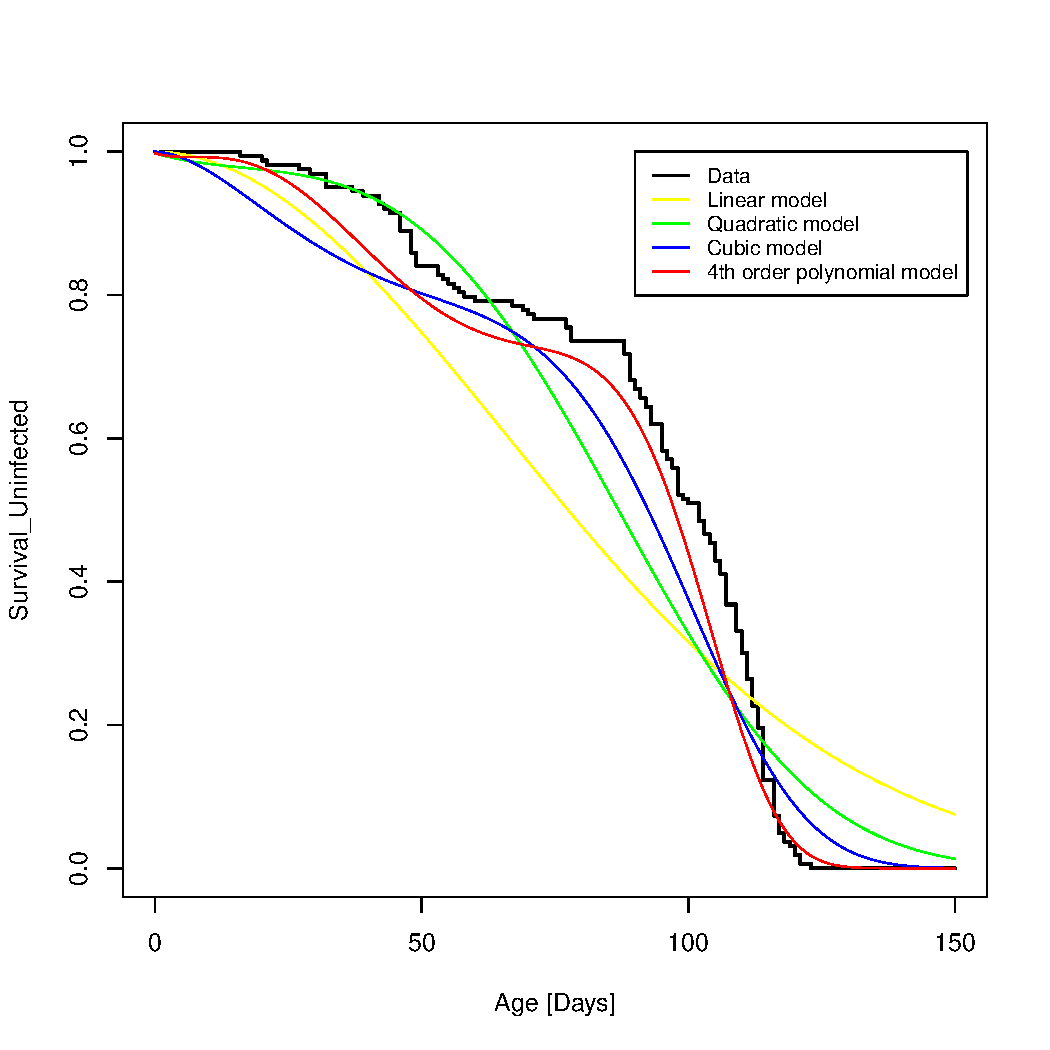
\includegraphics[width=\textwidth]{uninfected_population_survival_and_fit.pdf}
  \caption{The survival curve of all of the uninfected individuals, with our polynomial fits, fitted since age = 16, since there were no deaths before}
  \label{fig:survival_uninfected}
\end{figure}}

Using the likelihood ratio test, we have confirmed that the 4th order polynomial is the closest fit from those we have tried. We therefore now have a good estimate of the hazard function corresponding to the natural death rate.

In order to have the reference natural moratality rate for each of the age-at-infection compartment, we have fitted the uninfected survival two more times (age at infection = 15 overlapped, with the fit we made in Figure~\ref{fig:survival_uninfected}), each time we fitted starting from the age at infection of the desired compartment. The rates obtained like this should not however differ much from the deathrate described as obtained from Figure~\ref{fig:survival_uninfected}, we compare them in the Figure~\ref{fig:comparison_different_baselines}

\begin{figure}
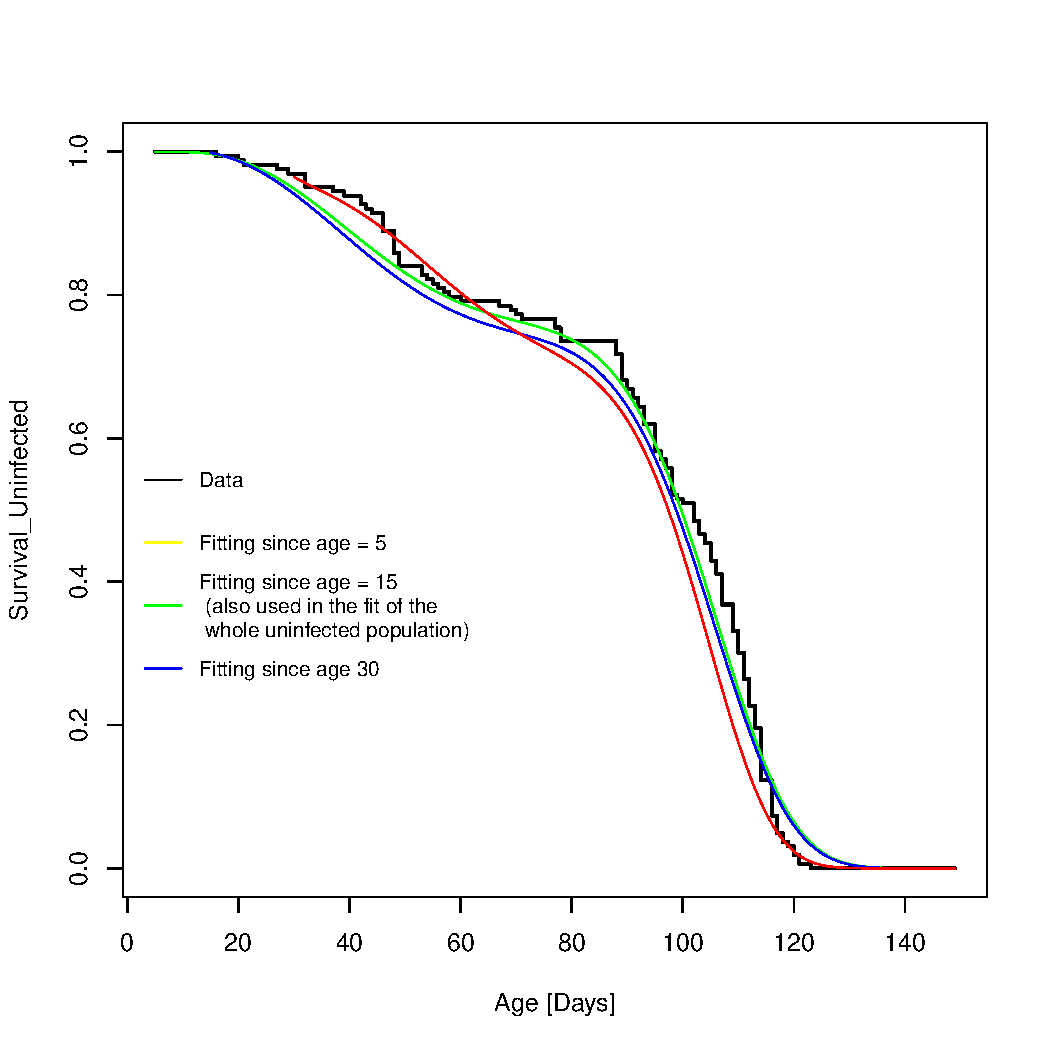
\includegraphics[width=\textwidth]{uninfected_population_survival_and_fit_different_starts_of_fitting.pdf}
\caption{Comparing the fitting of the survival of the uninfected population, using different starting points}
\label{fig:comparison_different_baselines}
\end{figure}

Even in these other cases, we concluded (using likelihood ratio test), that the best fit is the one assuming quartic polynomial for the hazard function.s

\subsection{Estimation of death rates in the infected population}

We then proceeded with estimating the death rate in populations with different age at infection. We obtained the plots in Figure~\ref{fig:survival_infected}

\textsc{\begin{figure}[H]
\begin{subfigure}[b]{0.5\textwidth}
    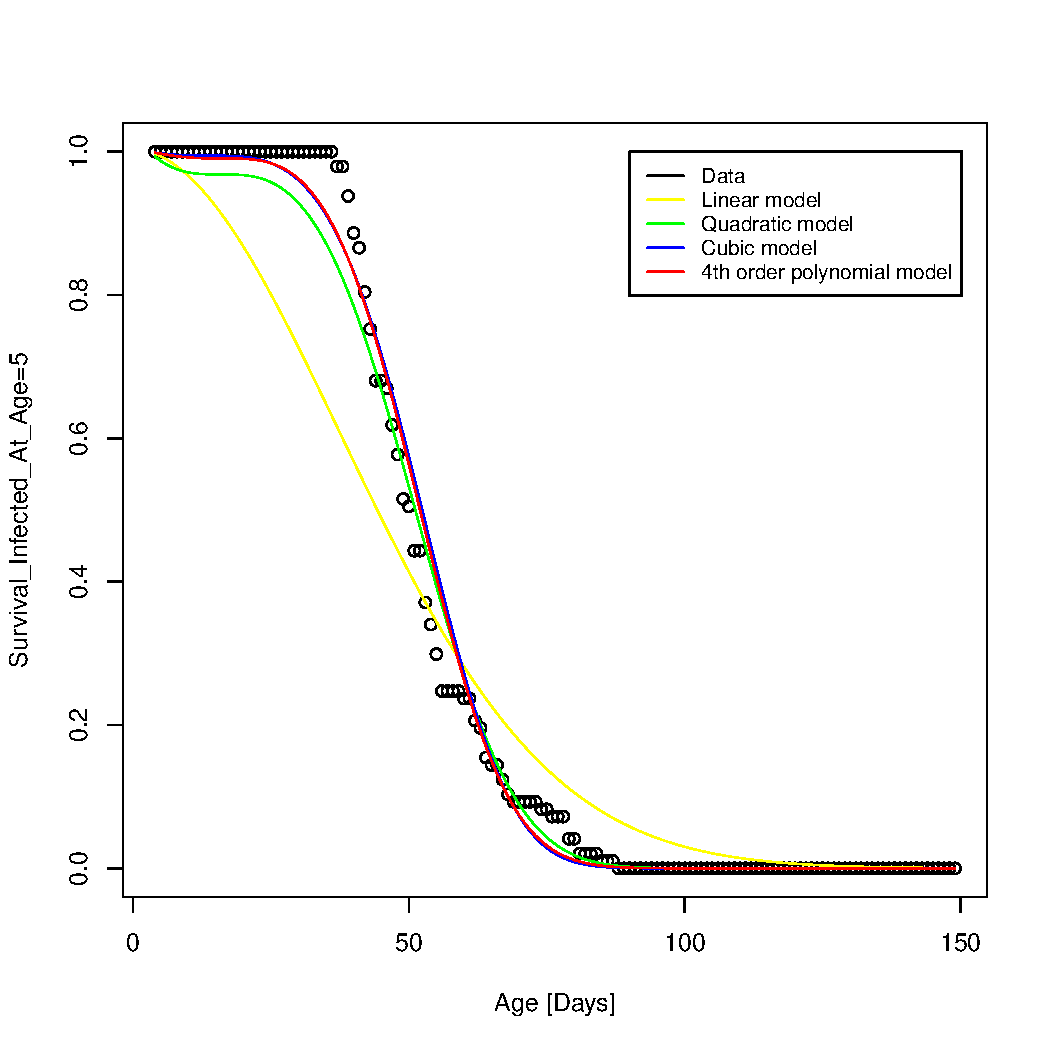
\includegraphics[width=\textwidth]{Fitting_delta_inf_at_age_5.pdf}
    \caption{Fitting the survival curve for age at infection = 5}
    \label{fig:subfigure_1}
  \end{subfigure}
  %
  \begin{subfigure}[b]{0.5\textwidth}
    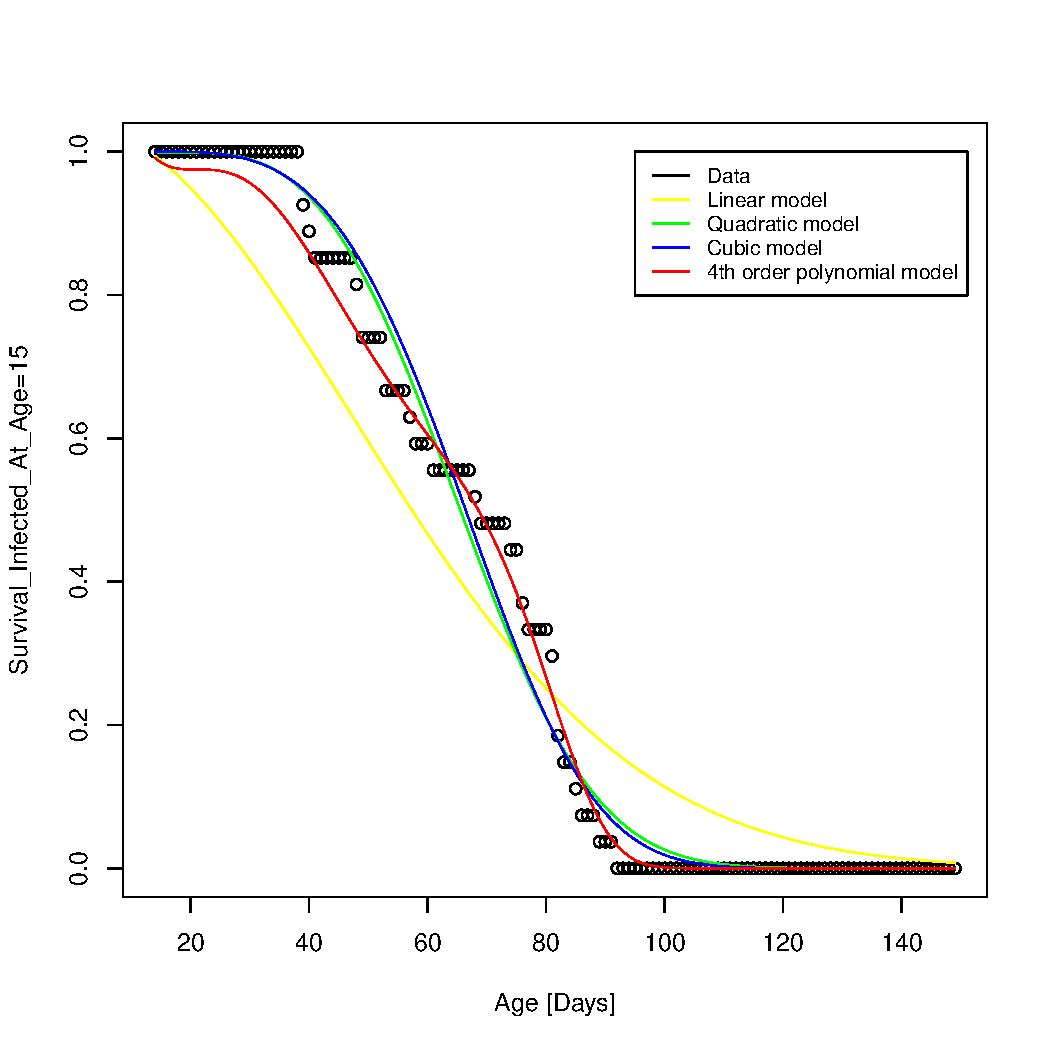
\includegraphics[width=\textwidth]{Fitting_delta_inf_at_age_15.pdf}
    \caption{Fitting the survival curve for age at infection = 15}
    \label{fig:subfigure_2}
  \end{subfigure}
  \begin{subfigure}[b]{0.5\textwidth}
    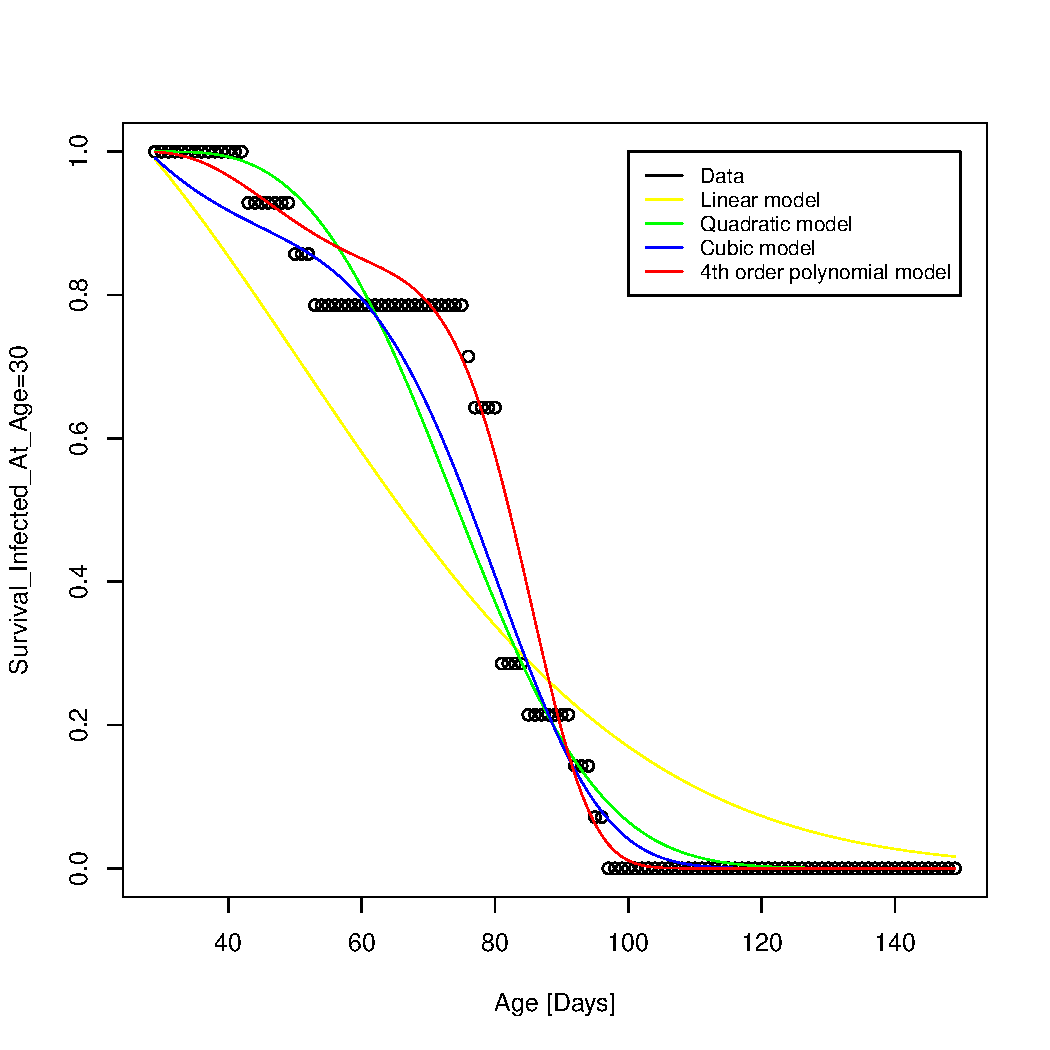
\includegraphics[width=\textwidth]{Fitting_delta_inf_at_age_30.pdf}
    \caption{Fitting the survival curve for age at infection = 30}
    \label{fig:subfigure_3}
  \end{subfigure}
  \caption{Survival curves in infected populations with different ages at infection, fitted everytime since the respective age at infection}
  \label{fig:survival_infected}
\end{figure}}

Using the likelihood ratio test, we have concluded that the quadratic fit was the best one in each of the cases.

\section{Virulence}

Using the hazard functions obtained in Section~\ref{natural_mortality}, we then constructed the virulence function for each age at infection. We constructed two versions, one using the identical natural death rate and one reflecting the different starting age for the fitting. We provide the plots corresponding to both of these versions in the Figure~\ref{fig:virulences}

\textsc{\begin{figure}[H]
\begin{subfigure}[b]{0.5\textwidth}
    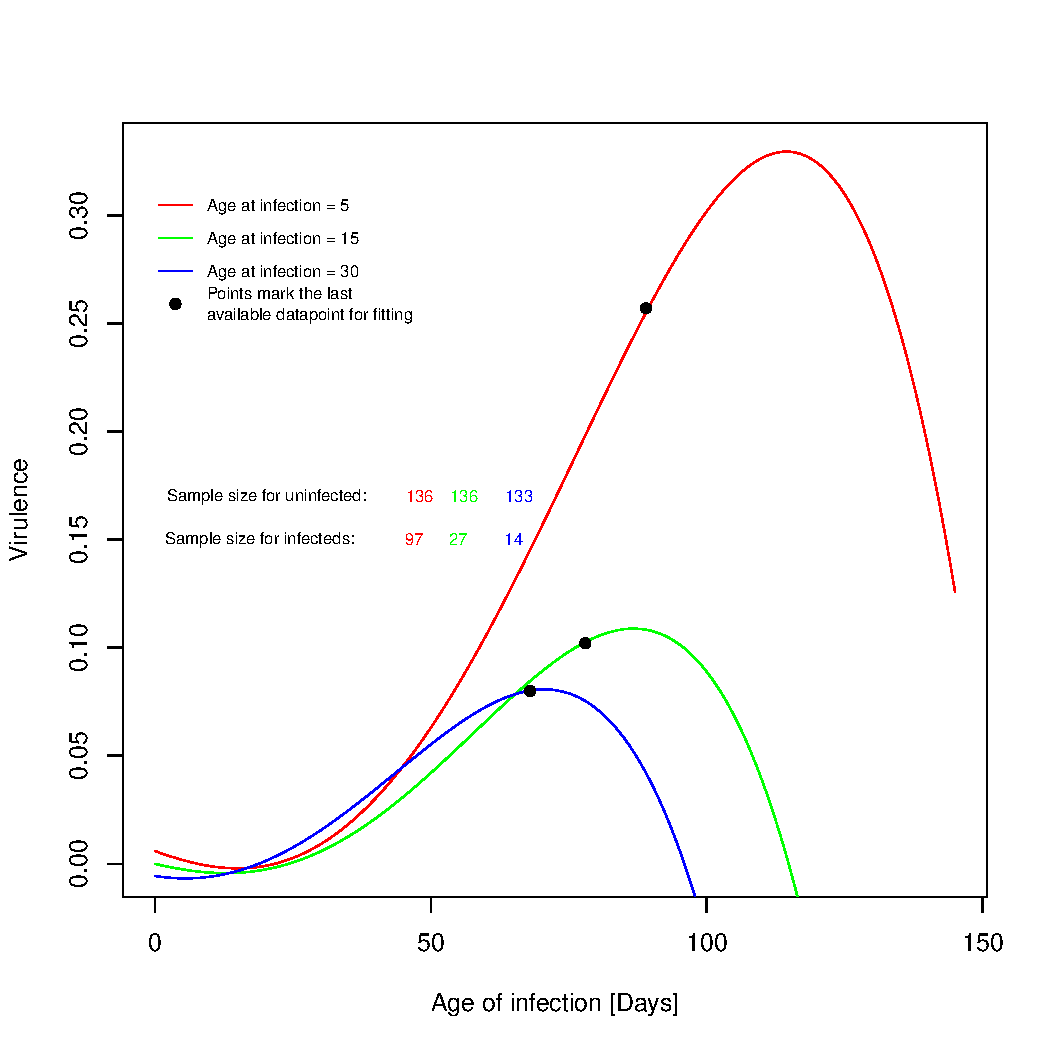
\includegraphics[width=\textwidth]{Virulences_age_of_infection_structured_same_baseline.pdf}
    \caption{Virulence computed using the same death rate in all age-at-infection compartments}
    \label{fig:subfigure_1}
  \end{subfigure}
  %
  \begin{subfigure}[b]{0.5\textwidth}
    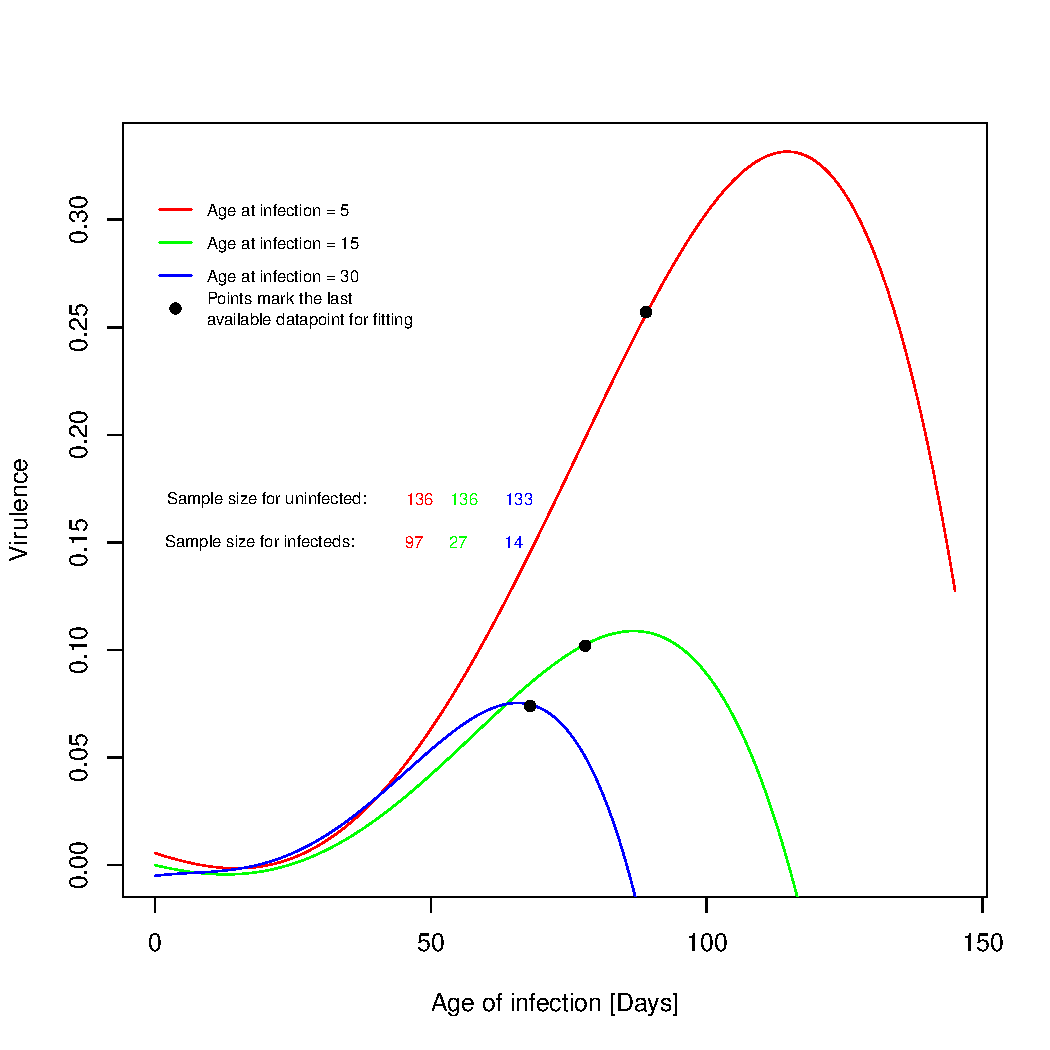
\includegraphics[width=\textwidth]{Virulences_age_of_infection_structured_same_model_for_same_infection_status.pdf}
    \caption{Virulence computed using the death rate fitted in each case since the respective age at infection}
    \label{fig:subfigure_2}
  \end{subfigure}
  \caption{Two versions of virulence}
  \label{fig:virulences}
\end{figure}}

We can see, that the virulence for the age at infection = 5 seems much higher then for the other ages, we would like to confirm this statistically now.\newline\newline
\textcolor{blue}{TODO: Test the hypothesis of the age-at-infection effect being significant}\newline
\textcolor{red}{Question: What kind of test to use?}


\bibliographystyle{unsrtnat}
\bibliography{bibliography_SIE_model}

\end{document}


